% !TeX spellcheck = en_US
\chapter{Our approach on the integration of Embree into ART}
\label{chap:math}

This section outlines our approach of the integration of Embree into ART. The language, in which the individual procedures are formulated is Objective-C, since the higher level functionality of ART has been written in this language, too. Embree itself is written in C and intended for the adaption to image synthesis environments being written in C/C++, which is the industry standard. However, due to Objective-C being a strict superset of C, these two languages can be intermixed seamlessly. Therefore, no issues concerning the cross-linking of C and Objective-C were discovered during the development.

\section{Design choices}

One important design choice was to abstract functionality regarding Embree inside a single class, which we gave the name \texttt{ArnEmbree}, conform to the naming convention of Objective-C classes in ART. Classes of type "\texttt{Arn<name>}" belong to the category of so-called "Scene graph classes", to which, according to our own opinion, the \texttt{ArnEmbree} class belongs the closest to. The main tasks of this class are the creation and deletion of an Embree device and an Embree scene, the adding of different scene geometry, and performing the intersection calculations with Embree. This class should act as a singleton object. To quote from the ART handbook: "Apart from this struct, [the \texttt{art\_gv} global variable] there are no genuine global variables in ART, only global constants" \cite[Chapter 4.1.2]{arthandbook}. The singleton object obviously contradicts this statement. The main reason for this design is to keep the functionality regarding Embree separate form the functionality of what we will from now on refer to as \emph{native ART}, the original Advanced Rendering Toolkit without the integration of Embree. During the initial phase of this project, it was not clear whether both the research question of this thesis ("Can the CSG operations of ART be implemented using Embree?") and the question of whether Embree could be integrated into ART at all could be positively answered. In case of our work being unsuccessful, this separation would ease the process of reverse engineering ART to its initial state.
In spite of this separation, an inclusion of the \texttt{ArnEmbree} singleton class to the \texttt{art\_gv} variable is possible and not too complicated.

Another design decision was to enable support of Embree only when the user provided the parameter flag \texttt{-e} or \texttt{--embree} when invoking \texttt{artist}, like so:

\begin{Verbatim}
$ artist foo_scene.arm -e
\end{Verbatim}

Initilally, the provision of a parameter flag was intended for easily switching Embree support on and off in order to draw comparisons between the performances of ART with and without the help of Embree. However, this turns out to be still valuable, because certain scenes will be rendered faster with Embree and some will not. We will turn to this circumstance in more depth when discussing the results in Chapter \ref{chap:results}. 

Once the command line arguments of \texttt{artist} are evaluated, the \texttt{ArnEmbree} singleton class object, which we call "\texttt{embreeManager}", is initialized and set up, if the parameter flag was provided. Otherwise, \texttt{embreeManager} is set to \texttt{NULL}. From this point on, the \text{ArnEmbree} singleton can be retireved from anywhere in the code and at any point of the action sequence by the instruction, shown in Listing \ref{lst:embree_manager}.

\begin{listing} 
	\begin{lstlisting}
	ArnEmbree * embree = [ArnEmbree embreeManager];
	\end{lstlisting}
	\caption{Retrieving the \texttt{ArnEmbree} singleton.}
	\label{lst:embree_manager}
\end{listing}


\begin{listing}
	\begin{lstlisting}
	 if( [ArnEmbree embreeEnabled] ) 
	 {
	 		// ...
	 }
	\end{lstlisting}
	\caption{Verifying if the \texttt{ArnEmbree} singleton was initialized.}
	\label{lst:check_embree}
\end{listing}

Furthermore, if the singleton was initialized and set up, another global boolean variable, indicating whether Embree is enabled or not, is set to true. The value of this boolean can be retrieved by calling a class method called \texttt{embreeEnabled}. An example of this is given in Listing \ref{lst:check_embree}.

\section{The \texttt{ArnEmbree} singleton class and the extension of the \texttt{RayCaster} object}

The \texttt{ArnEmbree}, which is inherited from the \texttt{ArcObject} base class in ART, is initially constructed the following way: Instance variables are provided to store a single \texttt{RTCDevice} and a single \texttt{RTCScene} object for Embree. Although the instantiation of multiple RTCScenes on a single RTCDevice is possible with Embree, we are considering only single scenes containing all scene geometry. Furthermore, in this class, methods are defined for initializing different geometry types for Embree, adding them to the RTCScene, and finally commiting the RTCScene, which will trigger the build of Embree's own spatial acceleration data structures. Due to these data structures, the creation of the KD tree native to ART is not necessary and can be discarded.

In order to perform the actual ray-intersection testing with Embree, a class method was added to the \texttt{RayCaster} class, which is called \texttt{getIntersectionListWithEmbree}. In case Embree support is enabled, this method is called. In this function, a given ray is converted to an \texttt{RTCRay} and Embree's native function for intersection testing, \texttt{rtcIntersect1()}, is called. Since ART only support the cast of single rays, as opposed to ray packets, functionality for casting ray packets with Embree is not considered. After the intersection testing is performed, the  \texttt{tfar} value is updated with the hit distance (will will remain \texttt{INFINITY} if no intersection was found), and the uv coordinates, surface normal, and shape associated with the hit geometry are stored in a \text{ArIntersectionList} data structure. From this point, the ray tracing process continues as usual until the next ray ray is cast into the scene.

\section{Initializing shapes for Embree}

ART supports a variety of different geometrical shapes. An overview of these shapes can be found in the "ARM File Reference Manual" \cite{artreferencemanual}. The shapes are divided by ART into two categories: \emph{Analytic shapes} and \emph{Simple indexed shapes}. Analytic shapes in ART are represented as outlined in Section \ref{sec:quadrics} of Chapter \ref{chap:fundamentals}. Simple indexed shapes on the other side are described by an array of vertices (or points in three dimensional space) associated with it and an array of indices (very similar to the triangle primitves in \emph{OpenGL}). In ART, two shapes, namely triangles and quadrangles are considered simple indexed shapes. Figure \ref{fig:shape_types} gives an overview over the categories of shapes in ART. This section describes the initialization of these shape types for Embree. For now, we will not consider the initialization of CSG geometry (see Figure \ref{fig:art_csg}), since Section \ref{sec:embree_csg} is dedicated to the description and rendering of this type with Embree.

\begin{figure}[!tbp]
	\centering
	\subfloat[Simple indexed shape: Triangle.]{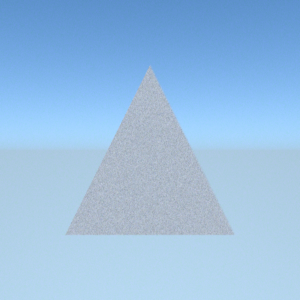
\includegraphics[width=.3\textwidth]{img/3 approach/triangle.png}\label{fig:art_triangle}}
	\hfill
	\subfloat[Analytical shape: Torus aligned on Y-axis.]{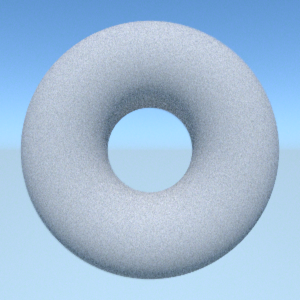
\includegraphics[width=.3\textwidth]{img/3 approach/torus.png}\label{fig:art_torus}}
	\hfill
	\subfloat[CSG geometry: Grooved sphere.]{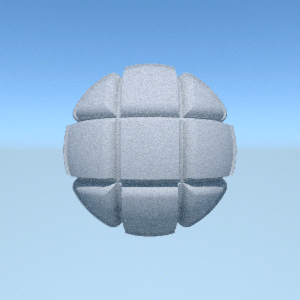
\includegraphics[width=.3\textwidth]{img/3 approach/csg_shape.png}\label{fig:art_csg}}
	\caption{Types of shapes in ART.}
	\label{fig:shape_types}
\end{figure}

Although it would be convenient to describe all shape types in ART as User defined geometry, we make the distinction between \emph{User defined geometry} and \emph{Non-user defined geometry}. Into the first category will fall the analytically described shapes. Triangles and quadrangles will be regarded as Non-user defined geometry and represented by Embree's own primitive types \texttt{RTC\_GEOMETRY\_TYPE\_TRIANGLE} and \texttt{RTC\_GEOMETRY\_TYPE\_QUAD}. This division makes sense, since the rendering of these primitive types with Embree is more efficient than User defined geometries. Furthermore, all the information needed to set up these primitive types are the vertices and indices associated with the primitive. They can be easily transferred from ART to Embree. 

The initialization of geometries for Embree takes place during the assembly of the scene graph from the information that have been parsed from the ARM scene file. At this step, the "Combined Attributes"- and "Shape"-node associated with the geometry are created and inserted to the graph as leafs. Additionally to this insertion, a class method of \texttt{ArnEmbree}, \text{initEmbreeGeometry()}, is called, and the shape object itself together with the newly created "Combined Attributes" node, the traversal state \todo{explain} of the RayCaster, the vertex set object containing the vertices of the shape, and finally, the transformation matrix are passed as funtion arguments. In this function, a new variable of the type \texttt{RTCGeometry} is being declared and initialized according to whether the shape is user-defined or not. The task of initializing geometries for Embree according to the category they belong to is performed by different class methods. After setting up a geometry for Embree, we are committing it, attaching it to Embree, and releasing it. When a geometry is successfully attached for Embree, a unique identifier is assigned to it. This identifier, and unsigned integer value, is refereed to as the \emph{Geometry ID}. We store this Geometry ID in an instance variable of the \texttt{Shape} and \texttt{Simple Indexed Shape} class. This identifier allows us, to retrieve the RTCGeometry from Embree and to perform alterations on it. However, the retrieving of RTCGeometry is only possible before the RTCScene is committed. \footnote{We actually not make use of this feature in the work this thesis describes, however, it may be useful to have for future work.}

\begin{listing} 
	\begin{lstlisting}
	// each geometry in the scene is associated with
	// this stuct, it is needed for embree to
	// perform user defined geometry intersection
	// calculations
	typedef struct GeometryData 
	{
		unsigned int _embreeGeomID; // geometry id of the shape
		ArNode * _shape; // ART's shape representation in memory
		ArTraversalState _traversalState; // state of the RayCaster
		
		ArNode<ArpRayCasting> * combinedAttributes; // node used for ray casting
		BOOL _isUserGeometry; // determines if geometry is User-defined or Non-user-defined
	}
	GeometryData;
	\end{lstlisting}
	\caption{\text{C} struct associated with each initialized geometry.}
	\label{lst:geometry_data}
\end{listing}

Once a geometry is attached to Embree, a \text{C} struct associated with the geometry in question is dynamically allocated ans stored in a linked list, whose head is an instance variable of the \texttt{ArnEmbree} class. The interior variables of this struct are shown in Listing \ref{lst:geometry_data}. They store the geometry id associated with the shape, ART's representation of the shape in memory, the traversal state of the \texttt{RayCaster} object when the shape was inserted as a leaf node into the scene graph \todo{explain}, a "Combined Attributes" node which is used for performing the ray tracing, and a boolean variables indicating if the shape is user defined or not.


\subsection{Intitialization of simple indexed geometry}
Simple index geometries are initialized the following way: Inside the \text{initEmbreeGeometry()} function, another class method with the name \texttt{initEmbreeSimpleIndexedGeometry()} is called, with the shape object the vertex set, and the transformation matrix being passed as arguments. 

\begin{listing} 
	\begin{lstlisting}
	RTCGeometry newGeometry = NULL;
	float * vertices;
	unsigned * indices;
	
	// if the shape is a triangle, 
	// create a new geometry buffer with type
	// RTC_GEOMETRY_TYPE_TRIANGLE
	if([shape isKindOfClass: [ArnTriangle class]]) 
	{
	
		newGeometry = rtcNewGeometry(device, RTC_GEOMETRY_TYPE_TRIANGLE);
		
		vertices = (float *) rtcSetNewGeometryBuffer(
													newGeometry,
													RTC_BUFFER_TYPE_VERTEX,
													0,
													RTC_FORMAT_FLOAT3,
													3*sizeof(float),
													3
													);
		
		indices = (unsigned *) rtcSetNewGeometryBuffer(
		                        newGeometry,
		                        RTC_BUFFER_TYPE_INDEX,
		                        0,
		                        RTC_FORMAT_UINT3,
		                        3*sizeof(unsigned),
		                        1
		                        );
	
	}
	\end{lstlisting}
	\caption{Setting up geometry buffers for the vertices and indices of a triangle shape.}
	\label{lst:geometry_buffer}
\end{listing}

In the interior of this function, depending of the shape passed to it being a triangle or quadrange, the new RTCGeometry variable is initialized either with the geomtry type \texttt{RTC\_GEOMETRY\_TYPE\_TRIANGLE} or \texttt{RTC\_GEOMETRY\_TYPE\_QUAD}. Following this initialization is the creation and assignment of two so-called \emph{geometry buffers}, one for storing the vertices associated with the shape and one for storing its indices. Listing \ref{lst:geometry_buffer} shows how the function \text{rtcSetNewGeometryBuffer()} is used to achieve that for a triangle shape. As input parameters this function takes the RTCGeometry to which the geometry buffer is associated to, the buffer type, a buffer slot number (here 0), the specified format for the buffer (RTC\_FORMAT\_FLOAT3 and RTC\_FORMAT\_UINT3 in Listing \ref{lst:geometry_buffer}), a byte stride argument and the number of items that shall be stored in the buffer. 

The setup for the geometry buffers for quadrangle is almost identical, with the only exception being that the RTCGeometry is initialized with the geometry type \texttt{RTC\_GEOMETRY\_TYPE\_QUAD} and that the byte stride of the vertex buffer is four instead of three.

Once these buffers are initialized, the vertices stored in the vertex set and indices associated with the shape representation of ART are transfered to the slots of the vertex and index geometry buffers. In case the transformation matrix that was passed to the function is not \text{NULL}, the vertices, one by one, are multiplied with it before being transfered to the vertex buffer. Embree allows instancing of geometry, meaning that geometry in Embree can be translated, scaled, and rotated by refering to an instance stored in memory and applying these transformation to it. \todo{weird sentence} However, we decided to perform the transformation calculation for each vertex before the transfer to the vertex geometry buffer, because this is more intuitive and easier to facilitate.
The initialization of a triangle mesh, beeing parsed from a PLY file with the help of the "RPly" library \cite{rply2016} follows the same outline described for triangles and quadrangles, although triangle meshes do not fall into the category of simple indexed shapes. The only difference is that the number of items for Embree's vertex geometry buffer is set to the number of total triangles in the mesh.
After the setup of the geometry buffers, the newly created RTCGeometry is returned from this function and assigned to the RTCGeometry, created in the \text{initEmbreeGeometry()} function, followed by the allocation of a \texttt{GeometryData} struct and the setup of its variables. The \text{isUserGeometry} boolean variable is set to false.

\subsection{Initialization of User defined geometry}
Under this category fall any shape of ART other than trianlges, quadrangles and triangle meshes. These shapes shall be initialized with Embree's primitive type \texttt{RTC\_GEOMETRY\_TYPE\_USER}. For initializing this kind of geometry type, one needs to provide three functions that are used by Embree as callback functions: one for calculating the bounding box of the shape, one for performing the actual ray-primitive instersection testing and one for testing for occlusion. For the setup of these shapes, an RTCGeometry with the type \texttt{RTC\_GEOMETRY\_TYPE\_USER} is declared. Subsequent to this declaration, three plain \texttt{C} functions for calculating the bounding box, testing for intersection points and testing for occlusion are provied to Embree as callback functions.
These functions have the name \texttt{embree\_bbox()}, \texttt{embree\_intersect()}, and \texttt{embree\_occluded()}. For ray tracing purposes, only one function for inersection calculation and occlusion testing would be necessary since both operation are performed by ray casting. However, Embree strictly expects two speperate function, each with a predetermined arguments. In order to compensate for this, we use a strategy which was inspired by the source code of Mitsuba 2: We refractor the ray tracing functionality into a fourth function called \texttt{embree\_intersect\_geometry()}, which is called from both the \texttt{embree\_intersect()} and \texttt{embree\_occluded()} function. 
In the interior of the function \texttt{embree\_bbox()}, the bounding box for a shape in question is calculated and passed to Embree. \texttt{embree\_bbox()} will be called by Embree, once the RTCScene is committed. Based on the individual bounding boxes of the geometries in the scene, Embree will cunstruct its BVH. Once an intersection with such a bounding box is found during ray tracing, Embree will call the \texttt{embree\_intersect()} function, which performs the intersection testing between the ray and the shape that is associated with that bounding box.


\todo{bullet lists}

\subsection{Ray tracing with Embree}
\label{sec:embree_raycasting}

Once the geometries contained in a virtual scene are initilialized for Embree, and Embree's internal BVH has been created, the scene is ready to be ray cast with Embree. If Embree support is enabled by the providing of the \texttt{-e} flag, a member function of the \texttt{RayCaster} class with the name \texttt{getIntersectionListWithEmbree} is called, which takes an empty \text{ArIntersectionList} struct \todo{explain} as an argument. In the body of this function, an \texttt{RTCIntersectContext} \todo{explain} is set up and a \texttt{RTCRayHit}\todo{explain too!} struct is declared.
This is followed by the update of the \texttt{RTCRayHit}, which is a unification of an \texttt{RTCRay} and an \texttt{RTCHit} struct with the current state of the \texttt{RayCaster} object. The information of the \texttt{RayCaster} object that is being transfered to the \texttt{RTCRayHit} stuct contains the orientation and direction of the ray that is about to be cast into the scene, and the ID associated to the ray. The \texttt{tfar} value of is initialized with Objective-C's \texttt{INFINITY} macro and the \texttt{geomID} field of the \texttt{RTCHit} struct is initialized with the macro \texttt{RTC\_INVALID\_GEOMETRY\_ID}. As mentioned, \todo{mention this} Embree utilizes single precision floating point numbers for its internal calculations, whereas ART uses double precision floating point numbers. To compensate for visual artifacts in the final image, we do not intitialize the \texttt{tnear} value of the \texttt{RTCHit} with zero, we instead give it a little offset, to prevent intersection between a secondary ray and the same shape that was already hit. We found the value $1e-3f$ to be reliable. A comparision of an image, rendered with and without this offset is given by Figure \ref{fig:offset}.

\begin{figure}[!tbp]
	\centering
	\subfloat[Rendering a quad without offsetting the \texttt{tnear} value.]{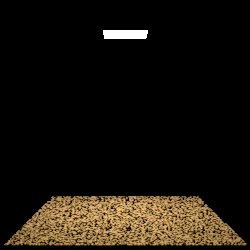
\includegraphics[width=.4\textwidth]{img/3 approach/artifact_2.png}}
	\hfill
	\subfloat[Rendering a quad with offsetting the \texttt{tnear} value by $1e-3f$.]{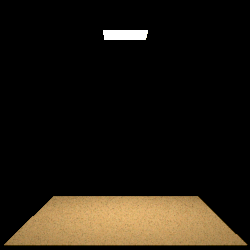
\includegraphics[width=.4\textwidth]{img/3 approach/artifact.png}}
	\caption{Artifacts due to the conversion of the hit distance of the ray from a double precision floating point number to a single precision floating point number.}
	\label{fig:offset}
\end{figure}

After the update of the \texttt{RTCRayHit} struct, the actual ray tracing is performed by calling the \texttt{rtcIntersect1()} function. Depending on whether a bounding box of a User geometry or Non-User geometry was hit with the \texttt{RTCRay}, either the provided callback function for intersecting User defined geometries, \texttt{embree\_intersect\_geometry()} or Embree performs the intersection testing with its own functionality. \todo{rephrase}


\subsubsection{Intersecting user defined geometry}
In case a bounding box of a user defined geometry is intersected with a ray by Embree, the provided callbak function \texttt{embree\_intersect\_geometry()} is getting called. In its interor, the \texttt{Geometry Data} struct associated with the geometry in question is retrieved from the geometry user pointer \todo{explain}. Subsequently, an empty \texttt{IntersectionList} \todo{explain} struct is declared and the intersection calulation with the ray and the shape is performed via calling the \texttt{getIntersectionList} function of the \texttt{Combined Attributes} object, which takes the intersection list as input, as well as the \texttt{RayCaster} object. This function will call the \texttt{getIntersectionList} function of the \texttt{Shape} object, which in return will calculate the intersection points on the shape and update the \texttt{IntersectionList} struct accordingly. The reason why this function is called on the higher level \texttt{Combined Attributes} object rather than directly on the \texttt{Shape} object is that by doing so, the transformation information of the shape will be taken into account.
If no intersection was found, we return immediately from the \texttt{embree\_intersect\_geometry()} function. Otherwise, we will update the \texttt{tfar} value of the \texttt{RTCRay} with the hit distance and the geometry ID of the \texttt{RTCHit} struct with the geometry ID associated with the intersected shape. 
The resulting intersection list is then stored in a linked list. 


\todo{inf sphere}


\section{Implementation of CSG operators to work with ART (WT)}
\label{sec:embree_csg}
\subsection{Approach 1}
\subsection{Approach 2}
\subsection{Approach 3}
